\chapter{TINJAUAN PUSTAKA}
\section{\textit{State of the Art}}
\noindent

\textit{State of the Art} Dalam penyusunan penilitian ini, peniliti mengambil beberapa referensi terdahulu sebagai panduan penulis untuk penilitian yang dilakukan, yang kemudian  akan menjadi acuan dan perbedaan dari penilitian yang akan dilakukan dengan penilitian sebelumnya. Pemaparan \textit{State of the Art} dapat dilihat pada tabel \ref{tb:stateoftheart} berikut.
\begin{landscape}	
	\pagestyle{empty}%
	\begin{center}
	\begin{longtable}{| c | L{3cm} | L{4cm} | L{2.5cm} | L{4cm} | L{3cm} | L{3cm} |}
	\caption{Paparan \textit{State of the Art}}
	\label{tb:stateoftheart} \\
	
	\hline 
	No &
	Penulis/Tahun &
	\multicolumn{1}{c|}{Judul Artikel} &
	\multicolumn{1}{c|}{Metode yang digunakan} &
	\multicolumn{1}{c|}{Hasil yang diperoleh} &
	\multicolumn{1}{c|}{Persamaan} &
	\multicolumn{1}{c|}{Perbedaan} \\ \hline
	\endfirsthead
	
	\hline 
	No &
	Penulis/Tahun &
	\multicolumn{1}{c|}{Judul Artikel} &
	\multicolumn{1}{c|}{Metode yang digunakan} &
	\multicolumn{1}{c|}{Hasil yang diperoleh} &
	\multicolumn{1}{c|}{Persamaan} &
	\multicolumn{1}{c|}{Perbedaan} \\ \hline
	\endhead
	
	\hline \multicolumn{7}{|r|}{{Bersambung}} \\ \hline
	\endfoot
	
	\hline \hline
	\endlastfoot
	1 	& Ibnu Ramadhan, Agung Purwanto dan Nurahman (2020) \cite{fps}
	& PENGEMBANGAN TEKNOLOGI \textit{GAME} INDONESIA UNTUK PERMAINAN \textit{FIRST PERSON SHOOTER} (FPS) 3D \textit{MULTIPLAYER} “CODE TO SHOOT” MENGGUNAKAN UNITY NETWORK (UNET) BERBASIS MOBILE
	& Unity Network
	& \textit{Game} ini dapat dimainkan secara \textit{multiplayer} tanpa perlu memasukan alamat IP karena fitur uNet dapat bekerja dengan baik. Selain itu \textit{game} ini juga sudah dapat dimainkan menggunakan platform mobile (Android)
	& Sama sama \textit{game} bergenre \textit{first person shooter}(fps)
	& Perbedaannya peniliti menggunakan unet sebagai \textit{multiplayer} platform
	\\ \hline
	2 	& Shena Star Sarwodi, Wibisono Sukmo Wardhono, Muhammad Aminul Akbar (2020) \cite{Sarwodi}
	& Penerapan \textit{Multiplayer} Pada Gim Tower Defense Menggunakan Photon Unity
	& Photon Unity Networking
	& Dengan menerapkan Photon Unity Networking pada gim tower defense maka dapat diimplementasikan sebuah fitur yang dapat meningkatkan interaktivitas dan ketertarikan pemain pada gim yaitu fitur \textit{multiplayer}
	&Persamaannya yaitu menggunakan unity photon.
	&Perbedaannya terdapat pada game yang diterapkan .
	\\ \hline

	3 	& Ryan Nanda Pratama,  Anton Siswo Raharjo Ansori, Ashri Dinimaharawati (2021) \cite{Ansori}
		& PEMBUATAN \textit{MULTIPLAYER} \textit{GAME} UCING BELING MENGGUNAKAN ASSET STORE MIRROR
		& Asset Mirror
		& Pada \textit{multiplayer} \textit{game} Ucing Beling dapat dimainkan secara realtime dan berjalan dengan sesuai yang diharapkan
		& Persamaannya sama sama \textit{multiplayer}.
		& Perbedaannya peniliti menggunakan asset store mirror sebagai \textit{multiplayer} platform
		\\ \hline	
	
		4 	& I Kadek Budi Suartama, I Gede Mahendra Darmawiguna, dan I Made Putrama (2020) \cite{Gebug}
		& PENGEMBANGAN GAME MULTIPLAYER PENGENALAN BUDAYA GEBUG ENDE SERAYA KARANGASEM BERBASIS ANDROID
		 & Metode pengembangan dalam penelitian ini menggunakan GDLC (Game Development Life Cycle)
		 & pengujian blackbox mendapatkan hasil bahwa semua fungsi dan fitur-fitur yang ada dapat 
		 berjalan dengan baik dan sebagaimana mestinya.
		 & Persamaannya yaitu menggunakan game engine unity.
		 & Perbedaannya terdapat pada metode yang digunakan.
		 \\ \hline

	
	
	5 	& Muhammad Faisal Fathurrohman Dan Iskandar Ikbal (2018) \cite{gogreen}
		& PEMBANGUNAN GAME MULTIPLAYER EDUKASI GO GREEN 3D BERBASIS ANDROID 
		& Google Play Games Realtime Multiplayer
		& Dapat terhubung secara multiplayer menggunakan google play games realtime multiplayer.
		&Persamaannya yaitu sama sama base multiplayer.
		&Perbedaannya terdapat pada google play games realtime multiplayer.
		\\ \hline
			  
	\end{longtable}
	\end{center}
	\end{landscape}

\section{Tinjauan Teoritis}
\subsection{Unity}
\noindent

Unity merupakan salah satu \textit{game} engine paling populer saat ini. Penggunaan Unity dapat digunakan untuk mengembangkan konten interaktif seperti video \textit{game}, 
visualisasi arsitektur, dan real-time 3D animasi. Unity menggunakan bahasa pemograman JavaScript dan 
C\# \cite{Ansori}. Unity juga merupakan perangkat lunak yang digunakan untuk mengembangkan \textit{game} \textit{multiplatform} yang didesain secara user \textit{friendly} 
(Iman, 2017). Keunggulan Unity adalah Unity 
dapat dengan mudah mengontrol objek-objek 
dalam gim atau aplikasi. Unity terdapat 2 jenis 
lisensi yaitu \textit{personal edition} yang dapat diakses 
secara gratis dan \textit{professional edition} yang 
diharuskan untuk membayar perbulan untuk 
mengaksesnya dengan beberapa fitur tambahan 
yang tidak terdapat di \textit{personal edition} \cite{Sarwodi}. 

\subsection{\textit{Multiplayer}}
\noindent

\textit{Multiplayer} merupakan fitur pada \textit{game} dimana pemain bermain dengan lebih dari 1 orang yang bermain 
di lingkungan \textit{game} yang sama dan waktu yang bersamaan. \textit{Game} \textit{Multiplayer} biasanya memberikan pilihan pada 
pemain untuk berbagi sumber daya sistem \textit{game} atau menggunakan internet untuk bermain bersama dalam jarak 
jauh. \textit{Game} \textit{Multiplayer} yang terhubung dengan internet melibatkan pemain yang saling terhubung melalui server. 
Sedangkan \textit{Game} \textit{Multiplayer} dengan koneksi lokal yaitu, pemain saling terhubung secara langsung dengan 
pemain lainnya, pemain terkoneksi menggunakan jaringan peer to peer. Pada \textit{Game} \textit{Multiplayer} online memiliki 
beberapa jenis kategori diantaranya adalah \textit{Massively} \textit{Multiplayer} Online \textit{game} (MMO), \textit{Massively} \textit{Multiplayer} 
Online \textit{First-person Shooter} \textit{Game} (MMOFPS), \textit{Massively} \textit{Multiplayer} online \textit{Real-time Strategy} \textit{Game}
(MMORTS), \textit{Massively} \textit{Multiplayer} Online Role-playing \textit{Game}s (MMORPG), \textit{Multiplayer} Online Battle Arena
(MOBA)\cite{Ansori}. 

\subsection{Photon Unity Networking (PUN)}
\noindent

Photon adalah sebuah framework pengembangan \textit{game} \textit{multiplayer} \textit{real-time} yang cepat, ringan, dan fleksibel. Photon terdiri dari server dan beberapa SDK klien untuk platform utama.
Photon Unity Network (PUN) adalah solusi khusus Unity yang dihadirkan dengan tingkat yang lebih tinggi: matchmaking, panggilan balik yang mudah digunakan, komponen untuk sinkronisasi \textit{Game}Objects, Remote Procedure Calls (RPCs), dan fitur serupa yang memberikan awal yang baik. Di luar itu, terdapat API yang solid dan luas untuk kontrol yang lebih canggih \cite{pun}.
Berikut gambaran 
integrasi aplikasi dengan Photon Unity Networking pada Gambar \ref{fig:photonni}
\begin{figure}[ht]
	\centering
	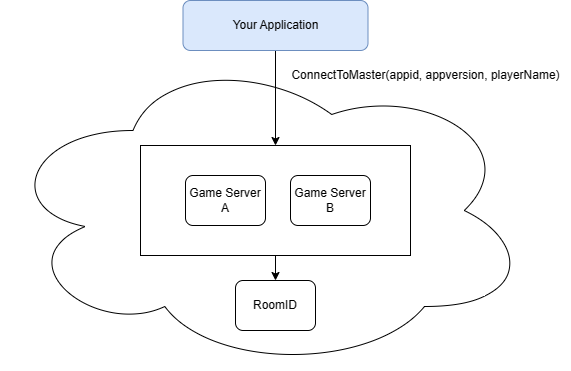
\includegraphics[width=10cm]{arsitektur-photon.png}
	\caption{Fitur Photon Unity Networking}
	\label{fig:photonni}
\end{figure}
\subsection{\textit{First Person Shooter}(FPS)}
\noindent

\textit{First Person Shooter} (FPS) adalah salah satu jenis \textit{game} yang saat ini sangat digemari terutama kalangan \textit{game}rs muda. FPS merupakan \textit{game} yang menggunakan sudut pandang orang pertama dimana pemain akan dibuat seolah-olah menjadi karakter utama dalam \textit{game} dengan tampilan yang berpusat pada permainan disekitar senjata atau alat yang sedang digunakan \cite{fps}.

\textit{First person shooter} merupakan jenis 3D \textit{game} shooter yang menampilkan sudut pandang orang pertama dengan 
pemain yang melihat aksi melalui mata karakter permain. Tidak seperti orang ketiga yang terlihat dari bagian 
belakang atau samping, yang memungkinkan \textit{game}r untuk melihat karakter secara keseluruhan\cite{fps}.

FPS dikembangkan pada tahun 1973 melalui permainan ruang yang belum sempurna yaitu flight simulator, yang 
menampilkan sudut pandang orang pertama dengan mengarah lebih rinci ke simulator pesawat tempur, dikembangkan untuk pasukan AS pada akhir tahun 1970-an. Permainan ini tidak lagi tersedia untuk konsumen \cite{fps}.

\subsection{C\#}
\noindent

C\# (C-sharp) adalah salah satu bahasa pemograman yang menggunakan Framework .NET. Sama seperti 
bahasa lainnya, C\# memiliki aturan pada syntax dan kode-kode yang bisa digunakan dalam pembuatan aplikasi. 
C\# cocok untuk dipelajari untuk pemula karena aturan syntax-nya lebih sederhana dibandingkan bahasa 
pemograman lainnya \cite{Ansori}.

\subsection{Wireshark}
\noindent

Wireshark merupakan sebuah \textit{software} penganalisa jaringan yang paling dikenal. \textit{Software} ini 
sangat berguna dalam menyediakan jaringan dan protokol serta memberikan informasi tentang 
data yang tertangkap pada jaringan. Software wireshark dapat menganalisa transmisi paket data 
dalam jaringan, proses koneksi dan transmisi data antar komputer\cite{wireshark}.

\subsection{\textit{Quality Of Service (QoS)}}
\noindent

QoS (Quality Of Service) adalah parameter-parameter yang menjadi indicator bagus atau
tidaknya performansi dari suatu jaringan. Parameter
yang menjadi indikator dalam QoS ini meliputi 
Bandwidth, Troughput, dan \textit{Packet Loss}, delay, dan
jitter \cite{qos}. Untuk itu dilakukan analisis Quality Of
Service (QoS) pada jaringan photon cloud .Adapun 
standar pengkuran performansi dalam suatu jaringan 
yaitu TIPHON (Telecommunicationsand Internet 
Protocol Harmonization Over Networks) yang 
mengkategorikan beberapa performansi dalam 
perhintungan tertentu.

\begin{enumerate}
	\item \textit{\textit{Throughput}} \\
	\textit{Throughput} merupakan parameter QoS yang 
menunjukkan suatu kecepatan rata-rata bandwidth
yang sebenarnya, diukur dengan satuan waktu 
tertentu pada kondisi jaringan tertentu untuk 
melakukan pengiriman paket dengan ukuran tertentu 
juga. Hasil \textit{throughput} diambil dari jumlah paket 
data yang dikirim dibagi dengan jumlah waktu yang 
diperlukan saat pengiriman paket data.
	\item \textit{Packet Loss} \\
	\textit{Packet Loss} merupakan suatu parameter QoS 
yang menunjukkan suatu jumlah total keseluruhan 
paket hilang atau tidak sampai ke destinasi, 
dikarenakan adanya overload atau congestion pada 
jaringan. Dalam suatu jaringan, \textit{packet loss}
diwajibkan mempunyai persentase yang kecil sesuai 
dengan standar. 
\item \textit{Delay} \\
\textit{Delay} merupakan suatu parameter QoS yang 
menunjukkan jumlah waktu yang diperlukan paket 
untuk mencapai jarak dari source ke destination. 
Berberapa hal yang mempengaruhi delay adalah 
jarak, perangkat keras dan congestion. 
\item \textit{Jitter}\\
\textit{Jitter} merupakan suatu parameter QoS yang 
menunjukkan jumlah dari variasi-variasi delay pada 
transmisi paket pada jaringan. Hal ini disebabkan 
banyaknya variasi panjang antrian paket dalam 
waktu proses paket dan waktu penghimpunan ulang 
paket-paket.


\end{enumerate}





